\chapter{Week 4}
\section{Stationary Process Forecasting}
Suppose we observe a time series
$ X_1,\ldots,X_T $
that we believe has been generated by an underlying
stationary process. We would like to
produce an $ h $-step ahead
forecast
\[ \hat{X}_{T+h}=\hat{X}_{T+h\mid T}=f(X_t,\ldots,X_1) \]
forecasting $ X_{T+h} $. Ideally, $ \hat{X}_{T+h} $
would minimize the prediction error
\[ L(X_{T+h},\hat{X}_{T+h})=\min_f
    L(X_{T+h},f(X_{T},\ldots,X_1)) \]
where $ L $ is a loss function.

Frequently, the loss function is taken
to be the \emph{mean-squared error} (MSE)
\[ L(X_{T+h},\hat{X}_{T+h})=
    \E[\big]{(X_{T+h}-\hat{X}_{T+h})^2} \]
When using MSE, it is natural to consider
\[ L^2=\set{\text{Random variables } X: \E{X^2}<\infty} \]
$ L^2 $ is a Hilbert space when equipped
with the inner product
\[ \innerp{X}{Y}=\E{XY} \]
Hilbert spaces are generalizations of Euclidean space ($ \mathbf{R}^d $)
in which the geometry and notation of projection
are preserved.
\[ \Proj{X\to Y}=\innerp{X}{Y}Y \]
\begin{Definition}{Closed Linear Subspace}{}
    We say $ M\subseteq L^2 $
    is a \textbf{closed linear subspace}, if
    \begin{enumerate}[(i)]
        \item Linearity: $ X,Y\in M $, $ \alpha,\beta\in\mathbf{R} $
              then $ \alpha X+\beta Y\in M $
        \item Closed: If $ X_n\to X $ (in the sense that $ \E{(X_n-X)^2} \to 0 $),
              and $ X_n\in M $, then $ X\in M $.
    \end{enumerate}
\end{Definition}
\begin{Theorem}{Projection Theoren}{}
    If $ M $ is a closed linear subspace in $ L^2 $
    and $ x\in L^2 $, then there exists a
    unique $ \hat{X}\in M $ such that
    \[ \E{(X-\hat{X})^2}=\inf_{y\in M}\E{(X-Y)^2} \]
    Moreover, $ \hat{X} $ satisfies the prediction equations/normal
    equations:
    \[ (X-\hat{X})\in M^\perp \implies \E{(X-\hat{X})Y}=0\quad (\forall y\in M) \]
\end{Theorem}
In MSE forecasting, we want to choose
$ \hat{X}_{T+h} $ satisfying
\[ \E{(X_{T+h}-\hat{X}_{T+h})^2}=\inf_{y\in M}\E{(X_{T+h}-y)^2} \]
where $ M $ is a closed linear subspace based on the available
data.
\begin{enumerate}[(1)]
    \item $ M_1=\set{z:z=f(X_{T},\ldots,X_{1}), f\text{ is any
                  Borel Measurable function}} $
          In this case
          \[ \hat{X}_{T+h}=\E{X_{T+h}\mid X_{T},\ldots,X_1} \]
          Unfortunately $ M_1 $ is enormous and complicated!
    \item $ M_2=\Spanc{1,X_{T},\ldots,X_1}=
              \set{Y:Y=\alpha_0+\sum_{j=1}^{T} \alpha_j X_j,\,\alpha_0,\ldots,\alpha_T\in\mathbf{R}} $
          which is the linear functions of $ X_1,\ldots,X_T $.
          $ \hat{X}_{T+h} $ is called the \textbf{best linear predictor} (BLP).
\end{enumerate}
\section{Best Linear Prediction}
Suppose $ X_t $ is a (weakly) stationary time series.
Best linear prediction entails finding $ \hat{X}_{T+h} $ so that
\[ \E{(X_{T+h}-\hat{X}_{T+h})^2}=\inf_{y\in M_2}\E{(X_{T+h}-Y)^2} \]
$ \hat{X}_{T+h} $ is the best prediction among all linear
functions of $ X_T,\ldots,X_1 $.
\begin{Definition}{Projection}{}
    If $ \hat{X} $ satisfies
    \[ \E{(X-\hat{X})^2}=\inf_{y\in M}\E{(X-Y)^2} \]
    we say that $ \hat{X} $ is the \textbf{projection}
    of $ X $ onto $ M $, and we write $ \hat{X}=\Proj{X\onto M} $.
\end{Definition}
In particular, the BLP is
\[ \hat{X}_{T+h}=\Proj{X_{T+h}\onto M_2} \]
Consider the case when $ h=1 $. From the Projection Theorem, the BLP
is of the form
\[ \hat{X}_{T+1}=\phi_{T,0}+\sum_{j=1}^{T} \phi_{T,j}X_j \approx
    \phi_{T,0}+\sum_{j=0}^{T} \phi_{T,j}(X_j-\mu) \]
where $ \mu=\E{X_t} $. $ \hat{X}_{T+1} $ must satisfy
the \textbf{prediction equations},
\[ \E{(X_{T+1}-\hat{X}_{T+1})Y}=0\quad (\forall  Y\in M_2 ) \]
In particular,
\[ \E{(X_{T+1}-\hat{X}_{T+1})1}=0\quad(Y=1) \]
\[ \E{(X_{T+1}-\hat{X}_{T+1})X_j}=0\quad(1\le j\le T,\, Y=X_j) \]
We have $ T+1 $ equations. Since $ \E{X_{j}-\mu}=0 $,
\[ 0=\E{X_{T+1}-\hat{X}_{T+1}}=\mu-\phi_{T,0}+0\implies \phi_{T,0}=\mu \]
Before proceeding, note that this implies
\[ \E{(X_{T+1}-\hat{X}_{T+1})X_j}=\E{(X_{T+1}-\mu-(\hat{X}_{T+1}-\mu))(X_{j}-\mu)} \]
So we may assume WLOG that $ \mu=0 $, therefore $ \E{X_i X_j}=\gamma(j-i) $.
Therefore,
\[ 0=\E{(X_{T+1}-\hat{X}_{T+1})X_k}=\gamma(T+1-k)-\sum_{j=1}^{T} \phi_{T,j}\gamma(j-k)\quad(1\le k\le T) \]
Therefore, we have linear system of equations for $ \phi_{T,1},\ldots,\phi_{T,T} $:
\[ \sum_{j=1}^{T}\phi_{T,j}\gamma(j-k)=\gamma(T+1-k)  \]
Let
\[ \symbf{\gamma}_T=\begin{pmatrix}
        \gamma(T) \\
        \vdots    \\
        \gamma(1)
    \end{pmatrix}\in\mathbf{R}^T \]
\[ \Gamma_T=\bigl[\gamma(j-k),1\le j,k\le T\bigr]\in\mathbf{R}^{T\times T} \]
\[ \symbf{\phi}_T=(\phi_{T,1},\ldots,\phi_{T,T})^\top \in\mathbf{R}^T \]
this linear system may be expressed as
\[ \Gamma_T \symbf{\phi}_T=\symbf{\gamma}_T\implies \symbf{\phi}_T=\Gamma_T^{-1}\symbf{\gamma}_T \]
given that $ \Gamma_T $ is invertible.

The BLP is of the form
\[ \hat{X}_{T+1}=\symbf{\phi}_T^\top \symbf{X}_T=(\Gamma_T^{-1}\symbf{\gamma}_T)^\top \symbf{X}_T \]
where $ \symbf{X}_T=(X_{T},\ldots,X_1)^\top\in \mathbf{R}^T $.

When is $ \Gamma_T $ non-singular?
\begin{Theorem}{}{}
    If $ \gamma(0)>0 $, and $ \gamma(h)\to 0 $ as $ h\to\infty $, then
    $ \Gamma_T $ is non-singular.
\end{Theorem}
Takeaway: Most stationary processes (those whose serial dependence decays
over time) have non-singular $ \Gamma_T $.

Note that
\[ \hat{X}_{T+1}^2=\symbf{\gamma}_T^\top \Gamma_T^{-1}\symbf{X}_T \symbf{X}_T^\top
    \Gamma_T^{-1}\gamma_T \]
Note that $ \E{\symbf{X}_T \symbf{X}_T^\top}=\Gamma_T $.
Therefore, $ \E{\hat{X}_{T+1}^2}=\symbf{\gamma}_T^\top \Gamma_T^{-1} \symbf{\gamma}_T $.
Also, since
\[ \E{X_{T+1}\symbf{X}_T}=\symbf{\gamma}_T\implies
    \E{X_{T+1}\hat{X}_{T+1}}=\symbf{\gamma}_T^\top \Gamma_T^{-1}\symbf{\gamma}_T \]
It follows that the mean-squared prediction error is
\begin{align*}
    P_{T+1}^T
     & =\E{(X_{T+1}-\hat{X}_{T+1})^2}                                                                                       \\
     & =\E{X_{T+1}^2-2 X_{T+1}\hat{X}_{T+1}+\hat{X}_{T+1}^2}                                                                \\
     & =\gamma(0)-2 \symbf{\gamma}_T^\top \Gamma_T^{-1}\symbf{\gamma}_T+\symbf{\gamma}_T^\top \Gamma_T^{-1}\symbf{\gamma}_T \\
     & =\gamma(0)-\symbf{\gamma}_T^\top\Gamma_T^{-1}\symbf{\gamma}_T
\end{align*}
The mean-squared prediction error has a simple, computable
form depending on $ \gamma(h) $ for $ 1\le h\le T $.

\section{Partial ACF}
If $ X_t \sim \ARMA{p,q} $, then we might be able to identify
$ p,q $ by looking at the ACF\@.
\[ X_t \sim \AR{p}\implies\text{ACF has a geometric decay} \]
\[ X_t \sim \MA{q}\implies\text{ACF is non-zero at the first $q$ lags, then zero beyond} \]
ACF of an $ \ARMA{p,q} $ model can be calculated by calculating
the linear process coefficients $ \set{\psi}_{\ell=0}^\infty $.
Automated in R using \code{ARMAacf()}.
\begin{Definition}{Partial autocorrelation function}{}
    The \textbf{partial autocorrelation function} of a stationary
    process $ \set{X_t}_{t\in\mathbf{Z}} $ is
    \[ \phi_{h,h}=\Corr[\big]{X_{t+h}-\Proj{X_{t+h}\onto X_{t+h-1},\ldots,X_{t+1}},
        X_{t}-\Proj{X_t\onto X_{t+h-1},\ldots,X_{t+1}}} \]
    Interpretation: Autocorrelation between $ X_t $ and $ X_{t+h} $
    after removing the linear dependence on the intervening variables $ X_{t+h-1},\ldots,X_{t+1} $.
\end{Definition}
\begin{Remark}{}{rem_acf}
    If $ X_t \sim \AR{p} $, then $ \phi_{h,h}=0 $ for $ h\ge p+1 $.
\end{Remark}
\begin{Proof}{\Cref{remark:rem_acf}}{}
    If $ X_t \sim \AR{p} $, then $ X_{t+h}=\sum_{j=1}^{p} \phi_j X_{t+h-j} +W_{t+h} $.
    \[ \Proj{X_{t+h}\onto X_{t+h-1},\ldots,X_{t+1}}=
        \sum_{k=1}^{h-1}B_k X_{t+h-k}  \]
    and minimizes
    \begin{align*}
        \E*{\biggl(X_{t+h}-\sum_{k=1}^{h-1} B_k X_{t+h-k}\biggr)^{\!2}}
         & =\E*{\biggl(W_{t+h}+\sum_{j=1}^{p} \phi_j X_{t+h-j}
        -\sum_{k=1}^{h-1} B_k X_{t+h-k}\biggr)^{\!2}}                                                          \\
         & =\sigma_W^2+\E*{\biggl(\sum_{j=1}^{p} \phi_j X_{t+h-j}-\sum_{k=1}^{h-1} B_k X_{t+h-k}\biggr)^{\!2}}
    \end{align*}
    where the second term is minimized by setting $ \beta_j=\phi_j $ for $ 1\le j\le p $
    and $ \beta_j=0 $ for $ j\ge p $. Note that $ W_{t+h} $ is independent of other terms.
    Hence,
    \[ X_{t+h}-\Proj{X_{t+h}\onto X_{t+h-1},\ldots,X_{t+1}}=W_{t+h}\quad(h\ge p+1) \]
    Therefore,
    \[ \phi_{h,h}=\Corr{W_{t+h},X_t-\Proj{X_t\onto X_{t+h-1},\ldots,X_{t+1}}} \]
    which is independent by causality. Therefore, $ \phi_{h,h}=0 $.
\end{Proof}
\begin{Remark}{}{}
    It can be shown that if $ X_t \sim \MA{q} $ (invertible), then
    \[ \phi_{h,h}\ne 0 \]
    \[ \abs{\phi_{h,h}}=\mathcal{O}(r^h)\quad(0<r<1) \]
    which is geometric decay.
    \begin{center}
        \begin{tabularx}{0.5\linewidth}{@{}YYY@{}}
                       & ACF                      & PACF                     \\
            \midrule
            $ \MA{q} $ & Cuts off after lag $ q $ & Geometric decay          \\
            $ \AR{p} $ & Geometric decay          & Cuts off after lag $ p $
        \end{tabularx}
    \end{center}
\end{Remark}
\subsection*{Estimating the PACF}
Using the BLP theory,
\[ \hat{\phi}_{h,h}=(\hat{\Gamma}_h^{-1}\hat{\symbf{\gamma}}_h)(h) \]
where
\[ \hat{\Gamma}_h=\bigl[\hat{\gamma}(j-k),\, 1\le j,k\le h\bigr]\in\mathbf{R}^{h\times h} \]
\[ \hat{\symbf{\gamma}}_h=\bigl[\hat{\gamma}(1),\ldots,\hat{\gamma}(h)\bigr]\in\mathbf{R}^h \]

\section{ARMA Forecasting}
Suppose $ X_t $ follows a stationary and invertible $ \ARMA{p,q} $
model so that $ \phi(B)X_t=\theta(B)W_t $. Having observed
$ X_T,\ldots,X_1 $, we wish to predict $ X_{T+h} $.
\[ \hat{X}_{T+h}=\Proj{X_{T+h}\onto M_2}\approx \E{X_{T+h}\given X_{T},\ldots,X_1} \]
by causality and invertibility $ X_t \sim $ linear function of $ W_t $.

Furthermore,
\[ \hat{X}_{T+h}\approx \tilde{X}_{T+h}=\E{X_{T+h}\given X_{T},\ldots,X_1,X_0,\ldots} \]
which is geometric decay of the dependence on past values.

Since $ X_t $ is casual and invertible,
\[ X_t=\sum_{\ell=0}^{\infty} \psi_\ell W_{t-\ell} \]
\[ W_t=\sum_{\ell=0}^{\infty} \pi_\ell X_{t-\ell} \]
where $ \psi_0=\pi_0=1 $. Note that
$ \psi $'s and $ \pi $'s are computable by solving homogeneous
linear difference equations.

These representations imply,
\[ \text{Information in }(X_T,X_{T-1},\ldots)=\text{Information in }
    (W_T,W_{T-1},\ldots) \]
So
\[ \tilde{X}_{T+h}=\E{X_{T+h}\given X_{T},X_{T-1},\ldots}=
    \E{X_{T+h}\given W_{T},W_{T-1},\ldots} \]
\begin{align*}
    \tilde{X}_{T+h}
     & =\E*{\sum_{\ell=0}^{\infty} \psi_\ell W_{T+h-\ell}\given W_T,W_{T-1},\ldots}                                                     \\
     & =\E*{\sum_{\ell=0}^{h-1} \psi_\ell W_{T+h-\ell}\given W_T,\ldots}
    +\E*{\sum_{\ell=h}^{\infty} \psi_\ell W_{T+h-\ell}\given W_{T},\ldots}                                                              \\
     & =\sum_{\ell=h}^{\infty} \psi_\ell W_{T+h-\ell}                               & \quad & \text{since $ \psi_\ell W_{T+h-\ell}=0 $}
\end{align*}
Also, using invertibility,
\[ 0=\E{W_{T+h}\given X_T,X_{T-1},\ldots}=
    \E*{\sum_{\ell=0}^{\infty} \pi_\ell X_{T+h-\ell}\given X_T,\ldots} \]
by independence, and furthermore, with $ \pi_0=1 $ we have
\[ 0=\tilde{X}_{T+h}+\sum_{\ell=1}^{h-1} \pi_\ell \tilde{X}_{T+h-\ell}+
    \sum_{\ell=h}^{\infty} \pi_\ell X_{T+h-\ell} \]
Therefore,
\[ \tilde{X}_{T+h}=-\sum_{\ell=1}^{h-1} \pi_\ell \tilde{X}_{T+h-\ell}-
    \sum_{\ell=h}^{\infty} \pi_\ell X_{T+h-\ell} \]

\subsection*{Truncated ARMA Prediction}
\[ \hat{X}_{T+h}=-\sum_{j=1}^{h-1}\pi_j\hat{X}_{T+h-j}-\sum_{j=h}^{T+h-1} \pi_j X_{T+h-j}  \]
\textbf{Residuals}:
\[ \hat{W}_t=\phi(B)\hat{X}_t-\theta_1\hat{W}_{t-1}-\cdots-\theta_q \hat{W}_{t-q} \]
\textbf{Mean initialization}:
\begin{itemize}
    \item $ \hat{W}_t=0 $ for $ t\le 0 $ and $ t\ge T $.
    \item $ \hat{X}_t=0 $ for $ t\le 0 $ and $ t\ge T+1 $.
    \item $ \hat{X}_t=X_t $ for $ 1\le t\le T $.
\end{itemize}
\textbf{Estimator for} $ \sigma_W^2 $:
\[ \hat{\sigma}_W^2=
    \frac{1}{T} \sum_{t=1}^{T} \hat{W}_t^2 \]
\textbf{Mean Squared Prediction Error}:
Since $ \hat{X}_{T+h}\approx \sum_{j=h}^{\infty} \psi_j W_{t+h-j} $,
\[ P_{T+h}^T=\E*{(X_{T+h}-\hat{X}_{T+h})^2}
    =\E*{\biggl(\sum_{j=0}^{h-1} \psi_j W_{t-j}\biggr)^{\!2}}=\sigma_W^2 \sum_{j=0}^{h-1} \psi_j^2 \]
\textbf{Estimated Mean Squared Prediction Error}:
\[ \hat{P}_{T+h}=\hat{\sigma}_W^2 \sum_{j=0}^{h-1} \psi_j^2 \]
\textbf{Construction of Prediction Intervals}:
Since $ \hat{X}_{T+h}\approx \E{X_{T+h}\given X_T,\ldots} $,
\[ \E*{\hat{X}_{T+h}-X_{T+h}}=0\quad(\text{Tower Property}) \]
\[ \E*{(\hat{X}_{T+h}-X_{T+h})^2}=P_{T+h}^T \]
Hence
\[ \frac{\hat{X}_{T+h}-X_{T+h}}{\sqrt{\hat{P}_{T+h}^T}}  \]
is an approximately mean zero and unit variance random variable.

Suppose $ C_\alpha $ is the $ \alpha $-critical value of this random variable,
then
\[ \hat{X}_{T+h}\pm C_{\alpha/2}\sqrt{\hat{P}_{T+h}^T} \]
is an approximate $ (1-\alpha) $ prediction interval for $ X_{T+h} $.

Choices for $ C_\alpha $:
\begin{enumerate}[(1)]
    \item $ Z_\alpha $ (standard normal critical value).

          Motivation: If $ W_t $ is Gaussian, then $ X_t=\sum_{\ell=0}^{\infty} \psi_\ell W_{t-\ell} $
          is Gaussian.
    \item Empirical critical value of residuals (standardized)
          \[ \frac{\hat{W}_{t}}{\sigma_W}\quad(1\le t\le T)  \]
    \item $ t $-distribution, Pareto, or skewed distribution fit to standardized residuals.
\end{enumerate}

\subsection*{Long Range Behaviour of ARMA Forecasts}
Suppose $ Y_t=s_t+X_t $ where $ X_t \sim \ARMA{p,q} $.
\[ \hat{Y}_{T+h}=\hat{s}_{T+h}+\hat{X}_{T+h}=\hat{s}_{T+h}+\Uunderbracket{\sum_{j=h}^{\infty} \psi_j W_{T+h-j}}_{\to 0(\text{ geometrically})} \]
$ \hat{Y}_{T+h} $ is converging fast to $ \hat{s}_{T+h} $: better get the trend for
long range forecasts.
\[ P_{T+h}^T=\sigma_W^2 \sum_{\ell=0}^{h-1} \psi_\ell^2\to \sigma_W^2 \sum_{\ell=0}^{\infty} \psi_\ell^2=\gamma_X(0) \]
In the long run, the MSE is the variance of $ X_t $.

\section{ARMA Forecasting Example 1: Cardiovascular Mortality}
\subsection*{Slide 1}
Let's give ARMA forecasting a try on real data.

\subsection*{Slide 2}
\begin{figure}[H]
    \centering
    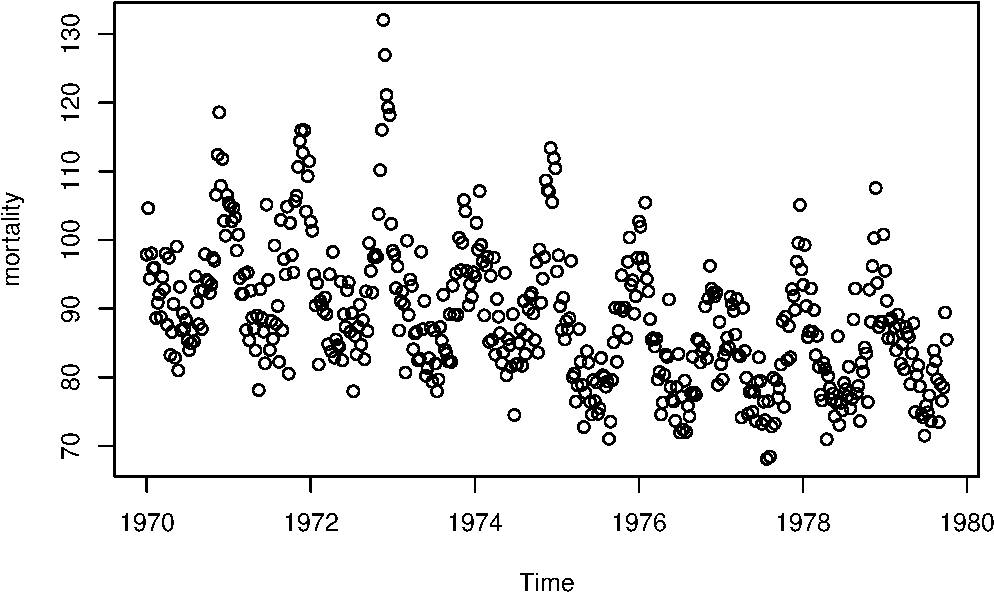
\includegraphics[width=0.7\textwidth]{wk_04-s_02.pdf}
    \caption{Weekly cardiovascular mortality, LA County.}
\end{figure}

\subsection*{Slide 3}
Let $ X_t= $ cardiovascular mortality series. Our model is
\[ X_t=s_t+Y_t \]
where $ Y_t \sim \ARMA{p,q} $.
\[ X_t=
    \Uunderbracket{\beta_0+\beta_1 t+\beta_2 t^2+\beta_3 t^3}_{\text{polynomial}}
    +\Uunderbracket{\beta_4\sin\biggl(\frac{2\pi}{52}t \biggr)
        +\beta_5\cos\biggl(\frac{2\pi}{52}t \biggr)+\beta_6\sin\biggl(\frac{2\pi}{26}t \biggr)
        +\beta_6\cos\biggl(\frac{2\pi}{26}t \biggr)}_{\text{seasonal}} \]
where the first four terms are the polynomial trends, the next two terms
are the yearly cycle, and the last two are the half-yearly cycle.

Decided on the trend using AIC, which will be discussed next week.

\subsection*{Slide 4}
$ s_t $ estimated using ordinary least squares.
\begin{figure}[H]
    \centering
    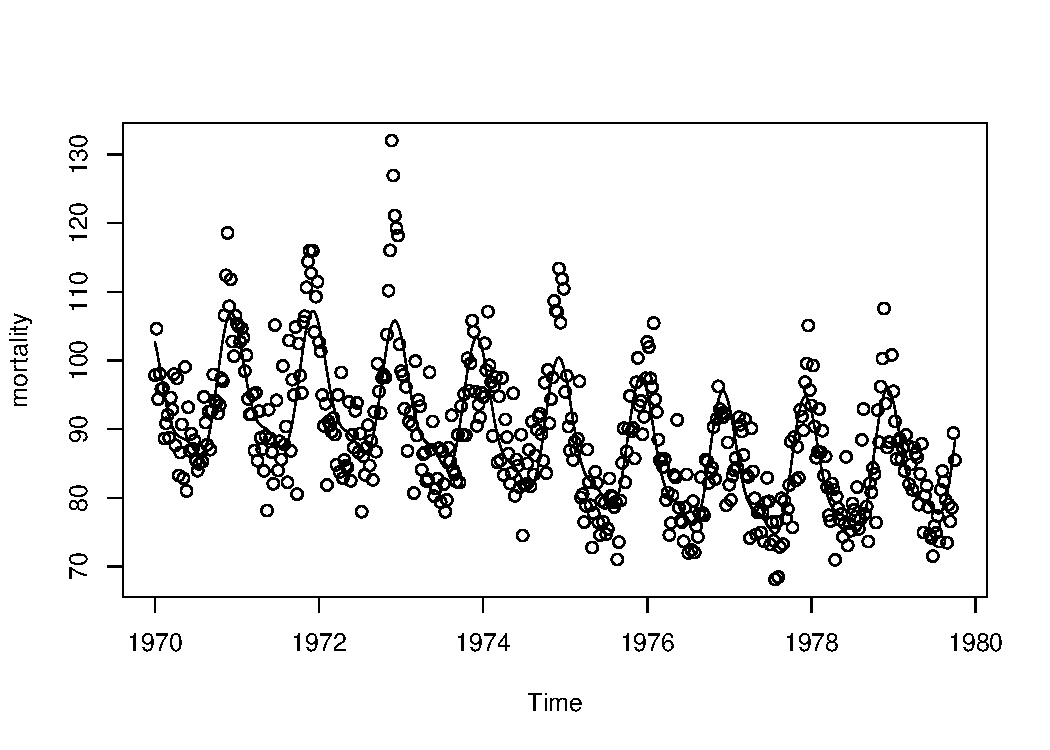
\includegraphics[width=0.7\textwidth]{wk_04-s_04.pdf}
\end{figure}

\subsection*{Slide 5}
\begin{figure}[H]
    \centering
    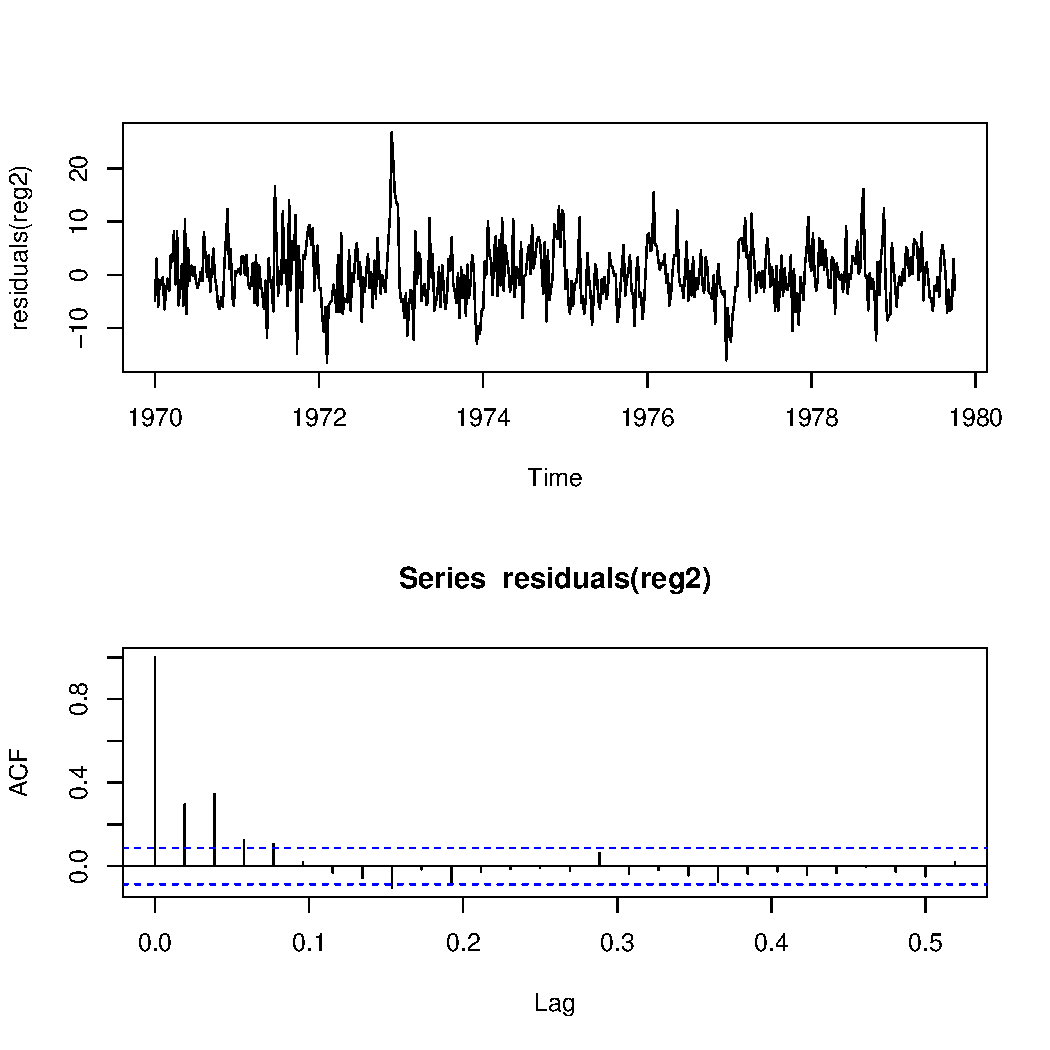
\includegraphics[width=0.7\textwidth]{wk_04-s_05.pdf}
\end{figure}
\begin{itemize}
    \item $ \hat{Y}_t=X_t-\hat{s}_t $ ``seems reasonably
          stationary.''
    \item Mild serial correlation in $ \hat{Y}_t $ --- Might be well modelled by $ \MA{2} $ or $ \ARMA{1,1} $.
\end{itemize}

\subsection*{Slide 6}
\begin{figure}[H]
    \centering
    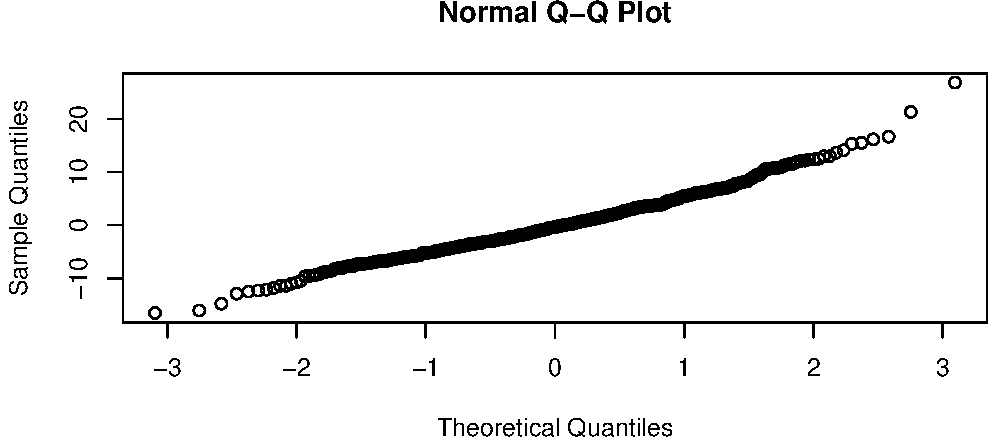
\includegraphics[width=0.7\textwidth]{wk_04-s_06.pdf}
\end{figure}
\begin{itemize}
    \item $ \hat{Y}_t $ seems reasonably normal, suggests
          using
          \[ \pm Z_{\alpha/2}\sqrt{P_{T+h}^T} \]
          to construct prediction bounds.
\end{itemize}

\subsection*{Slide 7}
\begin{figure}[H]
    \centering
    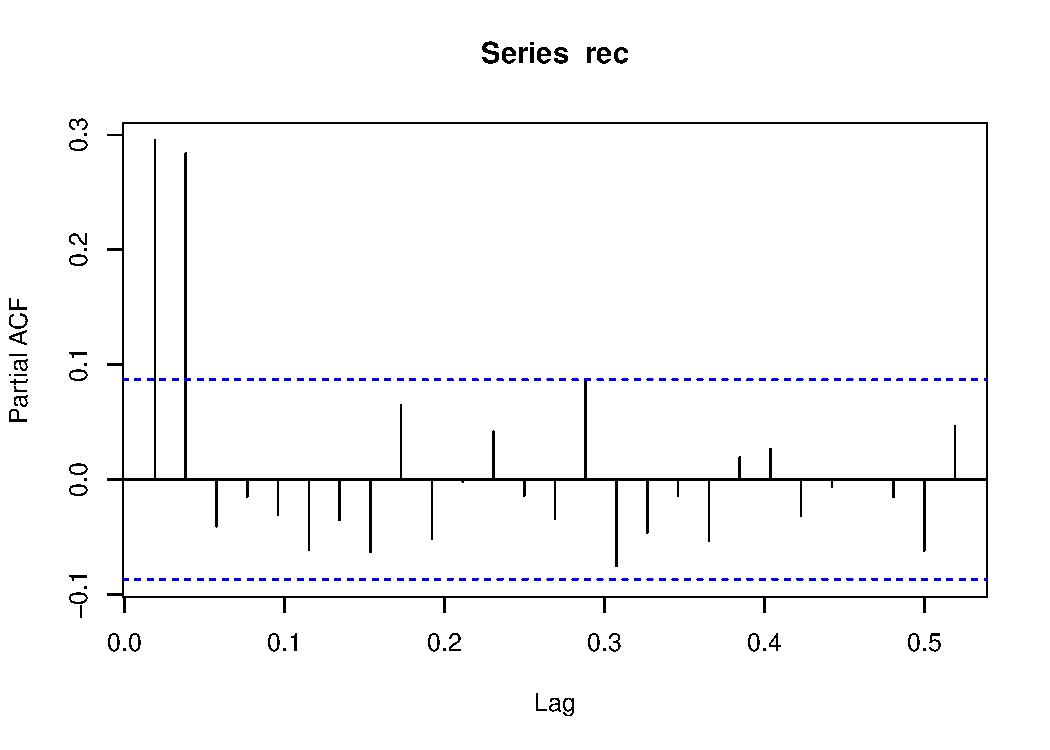
\includegraphics[width=0.7\textwidth]{wk_04-s_07.pdf}
\end{figure}
Considering the PACF\@: On the first two lags these are large which
is indicative of an autoregressive 2 structure, that is, $ \AR{2} $
structure.

\subsection*{Slide 8}
Model $ \hat{Y}_{t} $ as $ \ARMA{2,1} $.
\[ Y_t=0.0885 Y_{t-1}+0.3195 Y_{t-2}+W_t +0.1328 W_{t-1} \]
parameters estimated by MLE\@.

\subsection*{Slide 9}
\begin{figure}[H]
    \centering
    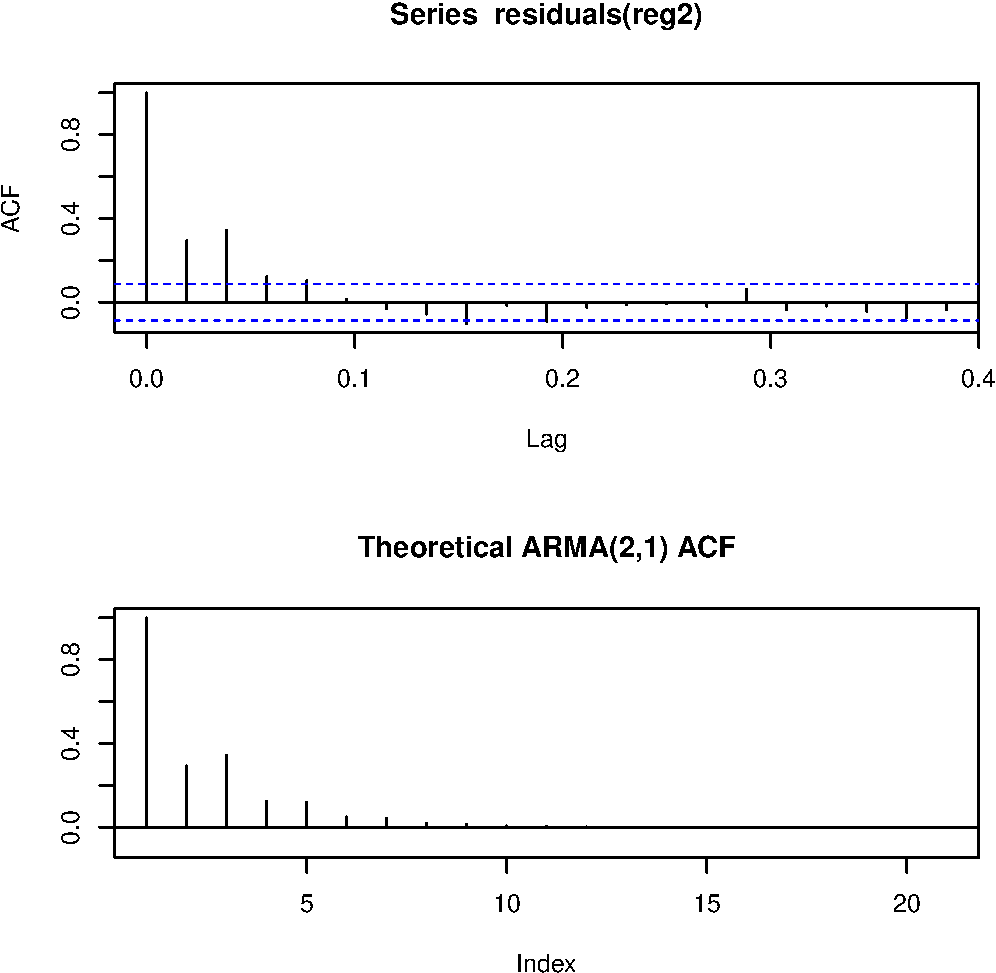
\includegraphics[width=0.7\textwidth]{wk_04-s_09.pdf}
\end{figure}

\subsection*{Slide 10}
\begin{figure}[H]
    \centering
    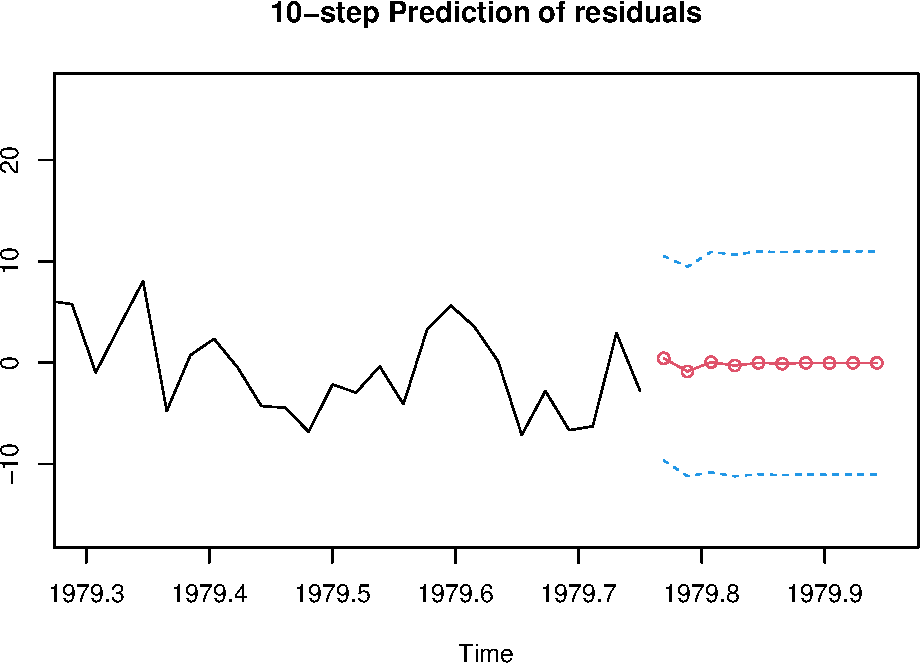
\includegraphics[width=0.7\textwidth]{wk_04-s_10.pdf}
\end{figure}
$ \hat{Y}_{T+h\mid T} $, $ h=1,\ldots,10 $.
\[ \hat{Y}_{T+h\mid T}\pm 1.96\sqrt{\hat{P}_{T+h}^T} \]
where $ 1.96 $ is the 97.5\% critical value of $ \N{0,1} $.

\subsection*{Slide 11}
\begin{figure}[H]
    \centering
    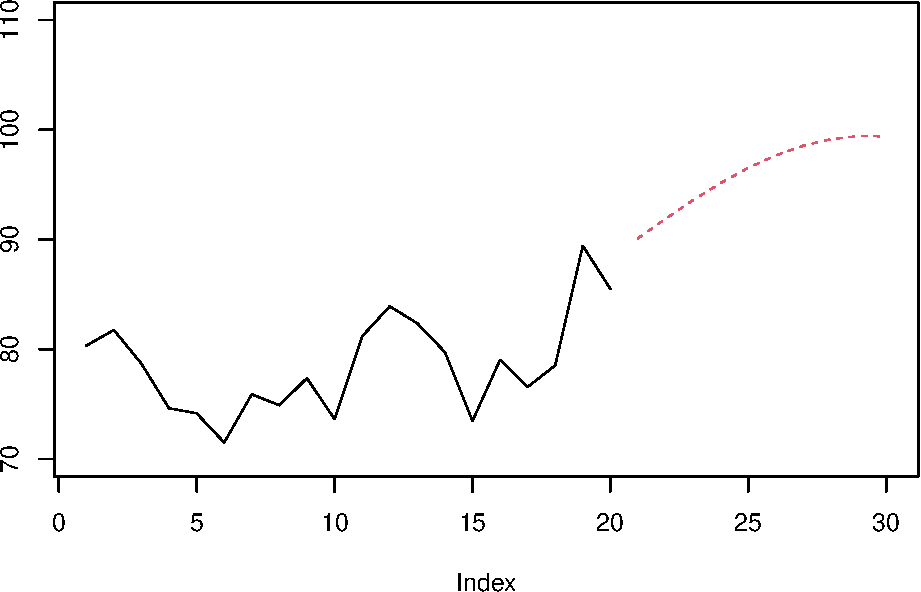
\includegraphics[width=0.7\textwidth]{wk_04-s_11.pdf}
    \caption{30 weeks of data with predicted trend}
\end{figure}

\subsection*{Slide 12}
\begin{figure}[H]
    \centering
    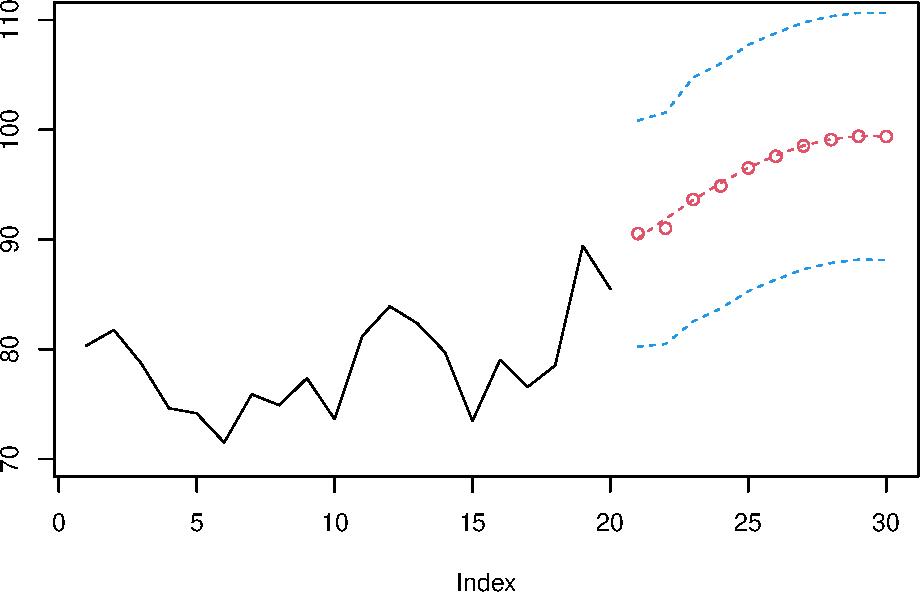
\includegraphics[width=0.7\textwidth]{wk_04-s_12.pdf}
    \caption{Forecasts with 95\% prediction intervals}
\end{figure}
Fluctuations attribute to serial dependence. Red lines
show that forecasts quickly converge to trend.

\begin{minted}{R}
####
##Cardiovascular Mortality Forecasting
#####

# SLIDE 1

# SLIDE 2
wk = time(cmort) - mean(time(cmort))  # wk is essentially t/52 centered at zero
wk2 = wk ^ 2
wk3 = wk ^ 3
cs = cos(2 * pi * wk)
sn = sin(2 * pi * wk)
cs1 = cos(4 * pi * wk)
sn1 = sin(4 * pi * wk)

reg2 = lm(cmort ~ wk + wk2 + wk3 + sn + cs + sn1 + cs1, na.action = NULL)
plot(cmort, type = "p", ylab = "mortality")

# SLIDE 3

# SLIDE 4
lines(fitted(reg2))

# SLIDE 5
par(mfrow = c(2, 1))
plot(residuals(reg2)) # \hat{Y}_t = X_t - \hat{S}_t "seems reasonably stationary"
acf(residuals(reg2))  # Mild serial correlation

# SLIDE 7
par(mfrow = c(1, 1))
rec = residuals(reg2)
pacf(rec)

# SLIDE 6 - Normal Q-Q Plot, stuff here
par(mfrow = c(1, 1))
qqnorm(rec)

# SLIDE 8
regr = arima(rec, c(2, 0, 1))
regr$coef

# SLIDE 9
par(mfrow = c(2, 1))
acf(residuals(reg2), 20, ylim = c(-.1, 1))
plot(
  ARMAacf(ar = c(0.0885,  0.3195), ma = c(0.1328), 20),
  type = "h",
  ylim = c(-.1, 1),
  main = "Theoretical ARMA(2,1) ACF",
  ylab = ""
)
abline(h = 0)

# SLIDE 10
par(mfrow = c(1, 1))
fore = predict(regr, n.ahead = 10)
ts.plot(
  rec,
  fore$pred,
  col = 1:2,
  xlim = c(1979.3, 1979.95),
  main = "10-step Prediction of residuals"
)
lines(fore$pred, type = "p", col = 2)
lines(fore$pred + qnorm(0.975) * fore$se,
      lty = "dashed",
      col = 4)
lines(fore$pred - qnorm(0.975) * fore$se,
      lty = "dashed",
      col = 4)

# SLIDE 11
inc = wk[2] - wk[1]
wkp = wk[length(wk)] + inc * (1:10)
wk = c(wk, wkp)
wk2 = wk ^ 2
wk3 = wk ^ 3
cs = cos(2 * pi * wk)
sn = sin(2 * pi * wk)
cs1 = cos(4 * pi * wk)
sn1 = sin(4 * pi * wk)

fit1 = 88.55365 - 2.96791228 * wk + 0.04624381 * wk2 +  0.09833614 * wk3 +  8.21611903 *
  cs +  4.08801987 * sn + 1.20542123 * sn1 + 2.77101452 * cs1
datl = rec + fit1[1:length(rec)]

plot(
  datl[(length(datl) - 19):length(datl)],
  xlim = c(1, 30),
  type = 'l',
  ylim = c(70, 110),
  ylab = ""
)
lines(21:30, fit1[(length(fit1) - 9):length(fit1)], col = 2, lty = 2)

# SLIDE 12
plot(
  datl[(length(datl) - 19):length(datl)],
  xlim = c(1, 30),
  type = 'l',
  ylim = c(70, 110),
  ylab = ""
)
lines(21:30, fit1[(length(fit1) - 9):length(fit1)], col = 2, lty = 2)
lines(21:30, fit1[(length(fit1) - 9):length(fit1)] + fore$pred, type = "p", col = 2)
lines(21:30,
      fit1[(length(fit1) - 9):length(fit1)] + fore$pred + 2 * fore$se,
      lty = "dashed",
      col = 4)
lines(21:30,
      fit1[(length(fit1) - 9):length(fit1)] + fore$pred - 2 * fore$se,
      lty = "dashed",
      col = 4)
\end{minted}

\section{ARMA Forecasting Example 2: Johnson and Johnson}
TODO a lot of practical stuff.
